%
%
%
\chapter{Spin-Fermion-Model}
\label{ch:spin fermion model}
%
%
%
The spin-fermion-model, as introduced in \cite{Abanov&Chubukov&Schmalian}, for a metal exhibiting a antiferromagnetic quantum phase transition is presented in following chapter.
Bosonic spin fluctuations arise in the vicinity of the quantum critical point due to fermionic particle-hole-excitations, enabling an attractive interaction between electrons.
This chapter does not intend to give a detailed mathematical and microscopic derivation of the spin-fermion-model.
It rather provides a qualitative description to justified the form of the model.
A short overview over quantum phase transitions is previously established, as suggested in \cite{SachdevQCP}.
In particular focus lies on the arising spin fluctuations and why these fluctuations carry large momentum $\vb{Q}$.
The damped spin density propagator and its perodicity is finally introduced.
The basic concepts of the hot-spot theory are additionally presented.
The proof of momentum and current conservation is shown for cases: excluded and included umklapp scattering.
%
%
\section{The Spin-Fermion-Model at the Onset of the Antiferromagnetic Quantum Phase Transition}
\label{sec:spin-fermion-model}
%
%
An antiferromagnetic phase transition is observed in many metals at a characteristic temperature $\mt{T}_{\mt{N}}$, the so-called N\'eel-temperature.
This temperature can be changed by tuning a certain parameter like the pressure in the system or doping in the material
The spins of lattice atoms are generally radomly ordered at $T > T_{\mt{N}}$.
When temperature comes below $T_{\mt{N}}$, spins are being ordered due to thermal fluctuations in such a way that nearest neighbours always point to the opposite directions.
A schematic and simplified phase diagram is depicted in figure \ref{fig:phase diagram}.
%
\begin{figure}[t]
	\centering
	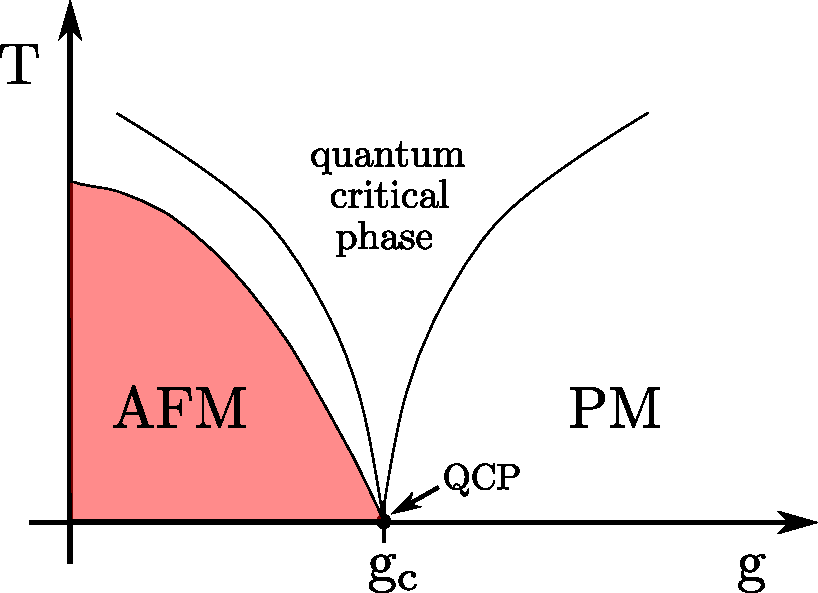
\includegraphics[width=0.6\textwidth]{phase_diagram.pdf}
	\caption{
A schematic and simplified phase diagram is shown for metals transition from a paramagnetic (PM) into an antiferrmagnetic (AFM) phase depending on a tunung parameter g.
The phase line of the AFM phase ends in a quantum critical point (QCP) at $\mt{g} = \mt{g}_{\mt{c}}$, decreasing temperature down to $T = 0$.
At this point, the phase transition is only caused by quantum fluctuations.
At $T > 0$, thermal fluctuactions more and more dominates the phase transition.
Nevertheless, the physical behaviour is influenced due to quantum fluctuations in a lagre regime, labeled as quantum critical phase.
	}
	\label{fig:phase diagram}
\end{figure}
%
The magnetic phase line ends at a certain value $\mt{g}_{\mt{c}}$ of the tuning parameter by decreasing the temperature up to $T=0$.
%A arbitrary point is considered on the phase line between both magnetic phases.
%This phase line ends at a certain value $\mt{g}_{\mt{c}}$ of the tuning parameter by decreasing temperature up to $T=0$.
This point is called quantum critical point due to the fact that the phase transition is originated by quantum fluctuation instead of thermal fluctuations.

A short describtion of quantum phase transitions is given and is continued by a qualitative derivation of the spin-fermion-model.
This overview is needed to understand the analytical discussion of our computation in chapter \ref{ch:calculation}.
The origin of phase transitions is always level crossing between the ground and an excited state.
A band gap $\Delta$ arises due to the fact that level crossing is forbidden.
This band gap is therefore a characteristic energy scale for the quantum phase transition.
The characteristic energy scale $\Delta$ is proportional to the tuning parameter
%
\begin{align}
	\Delta \sim \mt{J} |\mt{g} - \mt{g}_{\mt{c}}|^{z \nu},
	\label{eq:energy scale Delta}
\end{align}
%
considering only phase transitions of second order.
Here, $z\nu$ is a critical exponent and J an energy scale of a microscopic coupling \cite{SachdevQCP}.
A characteristic length scale $\xi$ is also required for quantum phase transitions.
This length scale is called correlation length, which diverges right at the quantum critical point.
%
\begin{align}
	\xi^{-1} \sim \Lambda |\mt{g} - \mt{g}_{\mt{c}}|^{\nu},
	\label{eq:correlation length xi}
\end{align}
%
where $\nu$ is again a critical exponent and $\Lambda$ an arbitrary inverse length scale as a momentum cut-off.
A directly relation between both characteristic quantities can be obtained when \eqref{eq:correlation length xi} is inserted in \eqref{eq:energy scale Delta}.
For finite temperatures, $T > 0$, a second energy scale is given by $k_{\mt{B}} T$, where $k_{\mt{B}}$ is the Botzmann constant.
A proportionality between temperatur and correlation length is
%
\begin{align}
	T \sim \xi^{-z}.
	\label{relation temperature and correlation length}
\end{align}
%
The curved conical boundary phase lines of the quantum critical phase can be explained with this relation.
Figure \ref{fig:phase diagram} shows this phase: In the case of small temperatures, the critical exponent $z$ attains the value $z = 2$, so that the phase lines are shaped like a square root.
At higher temperatures the phase boundary lines are linear, since the critical exponent is changed to $z = 1$ \cite{Patel&Sachdev}. 
In this regime the physical behaviour of metals is determined by quantum fluctions.

Now that the physical origin of quantum phase transitions is known, the spin-fermion-model is introduced.
Instead of a microscopic and detailed mathematical describtion, an introduction with qualitative arguments motivating the model is presented.
Metals in the vicinity of a magnetic quantum critical point are described with the spin-fermion-model, considering fermionic quasiparticles and bosonic spin density waves.
The fermionic propagator is determined by the usual free fermionic Green function.
Spin fluctuations are collective modes and their propagator is characterized by the dynamical magnetic susceptibility.
%
\begin{align}
	\mathcal{D}_{\mu}(\vb{q}, \omega) = \sum\limits_{\vb{Q}} \frac{1}{(\vb{q}+\vb{Q})^{2} + \xi^{-2} - (\flatfrac{\omega}{v_{\mt{S}}})^{2}},
	\label{eq:undamped spin propagator}
\end{align}
%
where $\mu$ is the spatial direction of the spin density wave, $\xi$ is the magnetic correlation length and $v_{\mt{S}}$ is the spin wave velocity.
The latter is of the same order as the Fermi velocity since spin fluctuations are originated due to fermions in the vicinity of the Fermi surface.
Furthermore, a peak at the momentum vector $\vb{Q} = (\pi, \pi)$ is exhibit in the magnetic susceptibility.
A strong coupling interaction is therefore implicated between momentum vectors $\vb{k}$ and $\vb{k} + \vb{Q}$.

Phase transitions are generally characterized by an order parameter. 
In the case of the investigated antiferromagnetic phase transition this also holds true.
The corresponding order parameter here is the local magnetization and can be measured by the spin expectation value $\expval{\vb{S}(\vb{r}_{i})}$.
Naturally, it is a sum over all spins located at a certain position $\vb{r}_{i}$.
The order parameter is finite in the antiferromagnetic ordered phase and vanishes in the paramagnetic disordered phase.
The expectation value of the spin operator is spatially modulated according to $\expval{\mt{S}_{\mu}} \sim \exp({i\vb{Q}\vb{R}})$, where $\vb{R}$ is a lattice vector \cite{Weiss}. 
As a consequence, the order parameter and equally the propagator are therefore periodic quantities.
This is reflected in the periodicity of the magnetic Brillouin zone, spanned by the vector $\vb{Q}$.

The presented describtion of the antiferromagnetic quantum phase transition in the spin-fermion-model is based on \cite{Abanov&Chubukov&Schmalian}.
It is assumed that spin fluctuations are generated over a large range of the tuning parameter g 
Other low-energy collective degrees of freedom that are independent of spin excitations are neglected.
At large values of the tuning parameter g in the paramagnetic phase, the physical behaviour is described by Landau's Fermi liquid theory.
Decreasing the tuning parameter and getting closer to the quantum critical point the behaviour is changed to a Non-Fermi liquid behaviour.
Only one type of fermions is assumed to be exist and the arising collective modes are originated from permanent interaction between particles and holes.
The physics in the vicinity of the quantum critical point is determined by spin excitations that are turning into smooth modes.
One dominant channel containing fermion-fermion interaction with energies smaller than a certain energy cut-off $\Lambda$ is assumed.

In the vicinity of the quantum critical point the (magnetic) correlation length $\xi$ and the coupling constant $\lambda$ is divergent.
The correlation length is therefore much larger than the lattice constant, $\xi \gg a$, and the coupling constant is much larger than the band gap, $\lambda \gg \Delta$. 
The band gap is associated with the energy of spin excitations.
In the limit of large distance and small energies or temperatures a mircoscopic consideration of the lattice Hamiltonian is unnecessary.
In this low-energy theory, spin fluctuations are described as a three component bosonic field $\Phi_{\mu}(\vb{x}, \tau)$.
The field is defined as a sum over all spin oparators analysed in the neighbourhood of the spin's position $i$.
It is formally writen as $\Phi_{\mu}(\vb{x}, \tau) \sim \sum_{i \in \Gamma(\vb{r}_{i})} \mt{S}_{\mu}(\vb{r}_{i})$, where $\mu$ is the spatial direction of the field and $\Gamma(\vb{r}_{i})$ represented the neighbourhood around the spin position $\vb{r}_{i}$ \cite{SachdevQCP}.
The magnitude of the bosnic field is chosen arbitrary and the field itself is considered as a real field.
The bosnoic field plays the role of an order paramtere, since the spin fluctuations only emerge near the phase transition.
In the low-energy theory, the obtained effective Hamiltonian for spin fluctuations is then given by
%
\begin{align}
	\mt{H}_{\Phi} &= 
	 	\sum\limits_{\mu} \int_{\vb{k}}\, \Big[
	 	-\frac{\vb{k}^{2}}{2} - \frac{r_{0}}{2}\Big] \Phi_{\mu}(\vb{k},\tau) \Phi_{\mu}(-\vb{k},\tau)
		+
		\frac{v_{\mt{S}}^{2}}{2} \pi_{\mu}(\vb{k},\tau) \pi_{\mu}(-\vb{k},\tau),
	\label{eq:Hamiltonian spin fluctuation}
\end{align}
%
where $r$ is a control parameter and corresponds to the squared inverse correlation length, $r = \xi^{-2}$.
The integral is extended over the first Brillouin zone and the sum runs over the spatial direction of the bosonic field.

It should be noted that the spin densiy waves are damped in consequence of the interaction with fermions.
The spin itself does not possess an own damping source.
The whole damping is governed by the decay of particel-holes-pairs.
As a consequence, the full renormalized particel-hole bubble corresponds to the inverse lifetime of spin fluctuations.
The interation Hamiltonian between spin density waves and fermions is given by
%
\begin{align}
	\mt{H}_{\Psi\Phi} &= 
		-\lambda \sum\limits_{\mu} \int_{\vb{k}} \int_{\vb{q}}\,
		\Phi_{\mu}(\vb{k}-\vb{q}, \tau)
		\bigg[
			\Psi_{\mt{a}}^{\dag}(\vb{k},\tau) \cdot \sigma_{\mu} \cdot \Psi_{\mt{b}}(\vb{q},\tau)
			+
			\Psi_{\mt{b}}^{\dag}(\vb{k},\tau) \cdot \sigma_{\mu} \cdot \Psi_{\mt{a}}(\vb{q},\tau)
		\bigg],
	\label{eq:Hamiltonian interaction}
\end{align}
%
where $\lambda$ is the coupling constant. 
Both integrals are extended over the first Brillouin zone and the sum runs over the spatial directions of the bosonic field.
$\sigma_{\mu}$ is the Pauli matrix with respect to the spatial direction.
The two different Fermi surfaces in the obtained model are represented by the indicies a and b at the fermionic fields $\Psi$.
%An detailed explanation is presently given below.
The imaginary part of the susceptibility has to be computed in the low-energy limit with tools of the quantum field pertubation theory.
An explicite calculation is presented in the appendix \ref{appch:propagator}.
Furthermore, the dynamic of the spin fluctuations is assumed to be governed by the low-energy fermions.
The $\omega^{2}$-term in the susceptibility \eqref{eq:undamped spin propagator} can be neglected \cite{Abanov&Chubukov&Schmalian} and at the vicinity of the quantum critical point the correlation length diverges, implying $\xi^{-2} \to 0$.
The damped magnetic susceptibility is then given by
%
\begin{align}
	\mathcal{D}_{\mu}(\vb{q}, i\omega_{n}) = \sum\limits_{\vb{Q}} \frac{1}{(\vb{q}+\vb{Q})^{2} + \gamma|\omega_{n}|},
	\label{eq:damped spin propagator}
\end{align}
%
where $\omega_{n}$ represent the bosonic Matsubara frequency.
Spin fluctuations are no independent degrees of freedom due to the fact that their damping is strongly connected to fermions.
The interaction between fermions on the Fermi surface seperated by the large vector $\vb{Q}$ constitutes in the damped susceptibility.
These points seperated by $\vb{Q}$ on the Fermi surface are called hot-spots in two dimensions and their theory is discussed next.
%
\begin{figure}
	\centering
	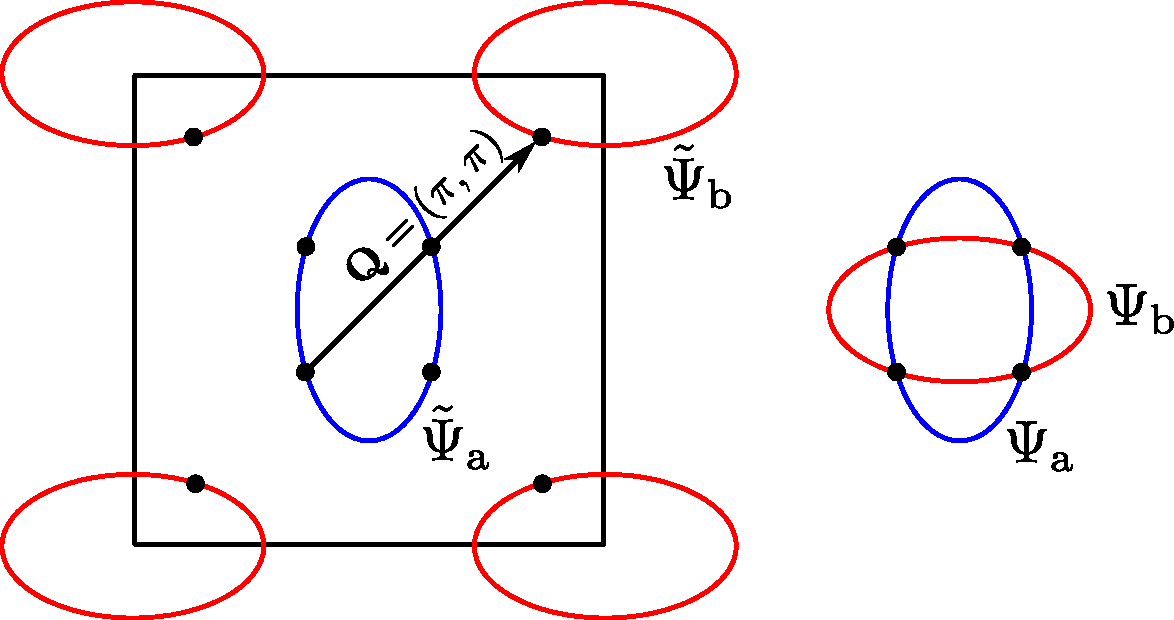
\includegraphics[width=0.6\textwidth]{hotspots.pdf}
	\caption{
One the left hand side the Brillouin zone is depicted containing the Fermi surface of both species of fermions, $\tilde{\Psi}_{\mt{a}}$ and $\tilde{\Psi}_{\mt{b}}$.
While the fermions $\tilde{\Psi}_{\mt{a}}$ are located with an anisotropic parapolical dispersion at the origin $(0,0)$, the fermions $\tilde{\Psi}_{\mt{b}}$ are located with a $\flatfrac{\pi}{2}$-rotated anisotropic parapolical dispersion at the corners of the Brillouin zone, $(\pi,\pi)$ for example.
The vector $\vb{Q}$ connects certain points on the Fermi surface, called hotspots and represented with dots. 
As a result of this an attraction between these fermions occurs.
On the right hand side the fermions $\tilde{\Psi}_{\mt{a}}$ are shifted to the corner at $(\pi,\pi)$.
The convienence of this represantation is that the coupling between fermions and spin fluctuations is local and independent of the position.
	}
	\label{fig:hotspots}
\end{figure}
%
In comparison to a normal metals, the new interaction of spin fluctuations seperates the Fermi surface in \emph{hot} and \emph{cold} manifolds.
A point $\vb{k}$ is considered on the Fermi surface of a $d$-dimensional system and, there, the fermion is assumed to has zero energy.
This point is connected to another point $\vb{k}+\vb{Q}$ via the spin density wave and is required to be also on the Fermi surface.
A $d-2$-dimension manifold is yielded for a $d$-dimensional system due to both constraints.
In the case of $d=2$ the \emph{hot} manifold is therefore called a hot-spot.
Another visualization of \emph{hot} manifolds is offered by the magnetic Brillouin zone spanned by the vector $\vb{Q}$.
The intersections of the magnetic Brillouin zone and the Fermi surface are equivalent to the \emph{hot} manifolds.

In our investigated model the fermions are considered as free, up to the interaction with the spin fluctuations.
Two species of fermions are assumed, $\tilde{\Psi}_{\mt{a}}$ and $\tilde{\Psi}_{\mt{b}}$. 
Their dispersion is anisotropic and parabolic, as suggested in \cite{Patel&Sachdev}. 
The anisotropic parabolic Fermi surface are depicted on the left hand side in figure \ref{fig:hotspots}.
This is not a discrepancy to our previous constraint, assuming one fermion, since both species of fermions are electrons and differ only in their dispersion.
The fermions $\tilde{\Psi}_{\mt{a}}$ and $\tilde{\Psi}_{\mt{b}}$ are located on an ellipse around the origin $(0,0)$ and $(\pi,\pi)$, respectivily.
Both ellipses are seperated by the vector $\vb{Q} = (\pi,\pi)$ and rotated by $\flatfrac{\pi}{2}$ to each other.
For achieving a continuum theory the ellipse centered around $(\pi,\pi)$ is shifted by the vector $\vb{Q}$ to the origin.
New fermionic fields, $\tilde{\Psi}_{\mt{a}}(\vb{r}) = \Psi_{\mt{a}}(\vb{r})$ and $\tilde{\Psi}_{\mt{b}}(\vb{r}) = \Psi_{\mt{b}}(\vb{r}) \exp(i\vb{Q}\vb{r})$, are therefore introduced.
The new Fermi surfaces of the fermions $\Psi_{\mt{a}}(\vb{r})$ and $\Psi_{\mt{b}}(\vb{r})$ are depicted on the right hand side in figure \ref{fig:hotspots}.
The enormous advantage of the continuum theory is that the coupling between the fermions, caused by spin density waves, is now local and indipendent of the position.
In reciprocal space, the Hamiltonian of the free fermions $\Psi_{\mt{a}}(\vb{r})$ and $\Psi_{\mt{b}}(\vb{r})$ is given by
%
\begin{align}
	\mt{H}_{\Psi} &= 
	 	\int_{\vb{k}}\,
	 	\bigg[
	 		\epsilon_{\mt{a}}(\vb{k})
	 		\psi_{\mt{a}}^{\dag}(\vb{k},\tau)
	 		\psi_{\mt{a}}(\vb{k},\tau)
	 		+
	 		\epsilon_{\mt{b}}(\vb{k})
	 		\psi_{\mt{b}}^{\dag}(\vb{k},\tau)
	 		\psi_{\mt{b}}(\vb{k},\tau)
	 	\bigg],
	 \label{eq:Hamiltonian electrons}
\end{align}
%
where the intergal is extended over the first Brillouin zone.
$\epsilon_{\mt{a}}(\vb{k})$ and $\epsilon_{\mt{b}}(\vb{k})$ are the anisotropic parabolical dispersions, corresponding to the fermion species a and b, and are given by
%
\begin{align}
	\epsilon_{\mt{a}}(\vb{k}) = \frac{k_{x}^{2}}{2m_{1}} + \frac{k_{y}^{2}}{2m_{2}} - \mu_{0}
	\qq{and}
	\epsilon_{\mt{a}}(\vb{k}) = \frac{p_{x}^{2}}{2m_{2}} + \frac{p_{y}^{2}}{2m_{1}} - \mu_{0},
	\label{eq:dispersion relations}
\end{align}
%
where $\mu_{0}$ is the chemical potential.
%
%
\section{Momentum Conservation in the Spin-Fermion-Model and the Consequence of Umklapp Scattering}
\label{sec:umklapp scattering}
%
%
In the low-energy theory, our investigated 2D-model is described by the continuum Hamiltonian $\mt{H}_{\Psi}$ for free fermions on the Fermi surface, the effective Hamiltonian $\mt{H}_{\Phi}$ for spin fluctuations and by the interaction Hamiltonian $\mt{H}_{\Psi\Phi}$ between both.
Directly at the quantum critical point the control parameter $r$ in \eqref{eq:Hamiltonian spin fluctuation} is zero, due to $r = \xi^{-2}$ and the correlation length $\xi$ is divergent.
$r$ is thus set to zero in the Hamiltonian $\mt{H}_{\Phi}$.
The obtained model Hamiltonian is given by $\mt{H} = \mt{H}_{\Psi} + \mt{H}_{\Phi} + \mt{H}_{\Psi\Phi}$.
In the next step, the conservation of momentum and current for this model Hamiltonian will be proved.
A pertubation Hamiltonian is then introduced to consider umklapp scattering, since translation symmetry is broken by this pertubation and momentum is not a conserved quantity any more.

A physical quantity is conserved, if its time derivative vanishes.
In quantum mechanics the time derivative is given by Heisenberg equation of motion, $\dot{\mt{A}}(t) = i\comm{\mt{H}}{\mt{A}(t)}_{-}$, where $\mt{A}(t)$ is an arbitrary operator.
The momentum operator is given by 
%
\begin{align}
	\mt{P}_{j} &= \int_{\vb{k}}\, 
		k_{j}\bigg[
	 		\Psi_{\mt{a}}^{\dag}(\vb{k},\tau) \Psi_{\mt{a}}(\vb{k},\tau)
	 		+
	 		\Psi_{\mt{b}}^{\dag}(\vb{k},\tau) \Psi_{\mt{b}}(\vb{k},\tau)
	 		-
	 		\pi_{\mu}(\vb{k},\tau) \Phi_{\mu}(-\vb{k},\tau)
		\bigg],
		\label{eq:momentum operator}
\end{align}
%
where the spatial direction is indicated by $j$.
The integral is extended over the first Brillouin zone and the sum over $\mu$ is implied in the last term.
The energy-momentum-tensor, as suggested in \cite{Iliev}, is used for the computation, shown in appendix \ref{appch:time derivative P and J}.
Further the x-component of current operator is given by
%
\begin{align}
	\mt{J}_{\mt{x}} &= - \int_{\vb{k}}\, \bigg[
		\frac{k_{\mt{x}}}{m_{1}} \Psi_{\mt{a}}^{\dag}(\vb{k},\tau) \Psi_{\mt{a}}(\vb{k},\tau)
		+ 
		\frac{k_{\mt{x}}}{m_{2}} \Psi_{\mt{b}}^{\dag}(\vb{k},\tau) \Psi_{\mt{b}}(\vb{k},\tau)
	\bigg],
	\label{eq:current operator}
\end{align}
%
where the integral is also extended over the first Brillouin zone.
The y-component of the current operator is obtained by changing the index x to y and interchanging the index a and b of the fermionic field operators.
Now, the time derivative of both quantities is computed by using the basic bosonic and fermionic commutator relations.
An explicite calculation is also represented in the appendix \ref{appch:time derivative P and J}.
This yields a vanishing time derivative for the the momentum,
%
\begin{align}
	\dot{\mt{P}}_{j} = 0,
	\label{eq:time derivative momentum}
\end{align}
%
and the following expression for the time derivative of the x-component of the current
%
\begin{align}
	\dot{\mt{J}}_{x} = \lambda
		\sum\limits_{\mu} \int_{\vb{k}} \int_{\vb{q}}\,
		\Phi_{\mu}(\vb{k}-\vb{q},\tau)
		\Big[
			&\Big(\frac{q_{\mt{x}}}{m_{1}} - \frac{k_{\mt{x}}}{m_{2}}\Big)
			\Psi_{\mt{b}}^{\dag}(\vb{k},\tau) \cdot \sigma_{\mu} \cdot \Psi_{\mt{a}}(\vb{q},\tau)
			\notag \\+
			&\Big(\frac{q_{\mt{x}}}{m_{2}} - \frac{k_{\mt{x}}}{m_{1}}\Big)
			\Psi_{\mt{a}}^{\dag}(\vb{k},\tau) \cdot \sigma_{\mu} \cdot \Psi_{\mt{b}}(\vb{q},\tau)
		\Big].
		\label{eq:time derivative current}
\end{align}
%
The y-component of the current is obtained by changing again the index x to y and interchanging the index a and b of the fermionic field operators.
In the spin-fermion-model, described by the Hamiltonian H, momentum is a conserved quantity, whereas the current is not.
The Hamiltonian is further invariant with respect to time reversal symmetry and a finite overlap is possessed between both quantities.
An infinite static electrical conductivity is obtained, compared to the discussion in chapter \ref{ch:infinite conductivity}.
A finite conductivity is only obtained when translation symmetry is broken.
This corresponds to an unconserved momentum.
Therefore, the model Hamiltonian H is pertubated by umklapp scattering via the Hamiltonian
%
\begin{align}
	\mt{H}_{\mt{umklapp}} = \sum\limits_{\mu, \vb{G}} \mt{J}_{\vb{G}}
		\int_{\vb{k}}\, \Phi_{\mu}(\vb{k},\tau) \Phi_{\mu}(-\vb{k}+\vb{G},\tau),
	\label{eq:Hamiltonian umklapp scattering}
\end{align}
%
where the integral extends over the first Brillouin zone and the sum over $\vb{G}$ includes all reciprocal lattice vectors.
The quantity $\mt{J}_{\vb{G}}$ is a coupling parameter depending on reciprocal lattice vectors.
It is assumed that the coupling is decreasing fast to zero in the limit of large reciprocal lattice vectors ($|\vb{G}| \to \infty$).
The time derivative of the momentum is given by
%
\begin{align}
	\dot{\mt{P}}_{j}(\tau) = i \sum\limits_{\vb{G}} \mt{J}_{\vb{G}} \int_{\vb{k}} G_{j} \Phi_{\mu}(\vb{k},\tau) \Phi_{\mu}(-\vb{k} - \vb{G},\tau)
	\label{eq:time derivative momentum finite}
\end{align}
%
with respect to the new model Hamiltonian $\mt{H}' = \mt{H} + \mt{H}_{\mt{umklapp}}$.
The time derivative of the current is persisted, since the current and pertubation Hamiltonian depends on different types of field operators and the commutator is therefore trivially zero.
The static electrical conductivity has become finite due to the unconserved momentum.
In the next chapter, the static electrical conductivity is computed using diagrammatic pertubation theory and the results are analysed.














